\label{chapter:preprocessor}

In this chapter, we present the first part of our system's pipeline: the \textsc{Preprocessor}. In order to avoid having to do extremely complicated semantic analysis in \textsc{SumASG}, we begin by pre-processing the input text so that we can give ASG something which is simpler to understand as well as more computationally tractable.

To ensure a consistent sentence structure for \textsc{SumASG}, we try and transform every sentence in the story to a basic subject-verb-object form (Section \ref{sec:tokenization_simplification}). To further help with the goal of generating optimal summaries, we take advantage of the \textsc{Preprocessor}'s semantic awareness to also remove irrelevant sentences and unnecessary use of synonyms (Section \ref{sec:pruning_homogenisation}). We illustrate how the \textsc{Preprocessor} works using our running example of the story of Peter Little (Section \ref{sec:preprocessor_example}).

\section{Overview}

The different stages of the \textsc{Preprocessor} can be seen in Figure \ref{fig:preprocessor_pipeline}. The first step is to \textit{tokenize} the story. After this we apply a number of transformations to reduce the complexity of the sentence structures. Once this \textit{simplification} step is complete, we prune away sentences which provide little value, and finally \textit{homogenise} the resulting text so that its lexical diversity is reduced.

{
\floatstyle{plain}
\restylefloat{figure}
\begin{figure}[H]
\centering
\begin{tikzpicture}[node distance=0.45cm, auto]
\node (story_in) [] {Story};
\node (tokenize) [block, right =of story_in] {Tokenize};
\node (simplify) [block, right =of tokenize] {Simplify};
\node (prune) [block, right =of simplify] {Prune};
\node (homogenise) [block, right =of prune] {Homogenise};
\node (story_out) [inter, right =of homogenise] {Pre-processed Story};
\draw [->] (story_in) -- (tokenize);
\draw [->] (tokenize) -- (simplify);
\draw [->] (simplify) -- (prune);
\draw [->] (prune) -- (homogenise);
\draw [->] (homogenise) -- (story_out);
\end{tikzpicture}
\caption{Preprocessor steps}
\label{fig:preprocessor_pipeline}
\end{figure}
}

\section{Tokenization And Simplification}
\label{sec:tokenization_simplification}

With the help of \textbf{CoreNLP}, we assign a POS tag to each word, or \textit{token}, from the input story. Using this information, we now make a number of simplifications which will make the sentence structure more consistent throughout.

\subsection{Punctuation}
\label{subsec:punctuation}

To avoid having to build recognition and semantic understanding of different types of punctuation into \textsc{SumASG}, it is preferable to transform the story such that it uses no punctuation apart from full stops. The idea is that each sentence in the resulting text contains exactly one action or description (i.e., it must consist of only one clause).

Depending on the type of punctuation used at the end of a clause in English, a different treatment is applied:

\begin{itemize}
\item Question marks: We remove the clause, as it is very uncommon for questions in a story to contain crucial information. It also helps avoid negation since we are deleting rhetorical questions.
\item Dashes: These are used around clauses which add detail, so it is quite safe to delete them for the task of summarization.
\item Exclamation marks, commas, semi-colons and colons: We replace any of these with a full stop.
\end{itemize}

\subsection{Individual Word Transformations}

One of the main goals of the \textsc{Preprocessor} is to transform the story into a simple and consistent structure, one where a given POS tag may only appear in a limited number of places in a sentence.

\subsubsection*{Acronyms, Contractions And Determiners}

Some acronyms are often spelled using full stops after each letter. To prevent these from being recognized as multiple sentences, it is beneficial to remove any punctuation from acronyms. For instance, the word ``U.S.A." becomes ``USA".

Contractions can be difficult to understand for machines, and they add unwanted complexity to the task of parsing. Therefore it is best to expand all of them, transforming ``it's" into ``it is".

In the English language, the determiners ``a" and ``an" are semantically identical, so it makes sense to only use one of the two to reduce the number of \textit{tokens} that \textsc{SumASG} has to process. After generating a summary, we will revert this change so that our framework's output is grammatically correct.

\subsubsection*{Adverbs}

In the English language, adverbs can appear almost anywhere in a sentence, and their position has minimal semantic influence. To illustrate this, consider the following sentences, which all have the same meaning:

\begin{displayquote}
\underline{Slowly} he eats toast. \\
He \underline{slowly} eats toast. \\
He eats toast \underline{slowly}.
\end{displayquote}

\noindent
In order to provide \textsc{SumASG} with a consistent format for parsing adverbs, we should always move them to the end of the clause in which they appear (in the above example we would keep the last sentence).

\subsubsection*{Possessive Pronouns, Interjections And Prepositions}

In most cases, possessive pronouns and interjections do not add much to the meaning of a story, especially when the end goal is to create a summary. Therefore, we remove such words from the text. For instance, the sequence ``\underline{Ah}! She ate \underline{her} chocolate." would become ``She ate chocolate.".

Prepositions which appear at the start of a sentence may be removed, as they are not integral to the meaning of the sentence. For example, ``\underline{Besides} today is Sunday" gets transformed into ``Today is Sunday".

Moreover, prepositions which come after the object in a sentence can sometimes cause it to become syntactically too complex. Rather than encoding such high level of detail into the internal representation of \textsc{SumASG}, it is preferable to simply omit the final clause. In this case, ``They have a picnic \underline{under} a tree." becomes ``They have a picnic.". Although some information is thrown away, and there could be a small impact on the quality of the summary, this is a simplification we are willing to make.

\subsection{Clause Transformations}

After going through the \textsc{Preprocessor}, we would like each sentence in the given story to only focus on a single topic.

When possible, we should split sentences containing multiple clauses into individual sentences. Otherwise, we delete the auxiliary clause to only keep the main clause. Examples of the transformations applied to different types of clauses can be seen below in Figure \ref{fig:clause_transformations}.

\begin{figure}[H]
\begin{subfigure}{\textwidth}
\begin{displayquote}
\textit{Conjunctive Clause}. We looked left \underline{and} they saw us.\\
\textit{Conjunctive Clause}. Cars have wheels \underline{and} go fast.\\
\textit{Subordinating Clause}. She never walks alone \underline{because} she is afraid.\\
\textit{Dependant Clause}. I want to be President \underline{when I grow up}.\\
\textit{Dependant Clause}. \underline{When I grow up}, I will have a garden.
\end{displayquote}
\caption{Before transformation}
\vspace{\baselineskip}
\end{subfigure}
\begin{subfigure}{\textwidth}
\begin{displayquote}
\textit{Conjunctive Clause}. We looked left. they saw us.\\
\textit{Conjunctive Clause}. Cars have wheels. Cars go fast.\\
\textit{Subordinating Clause}. She never walks alone. she is afraid.\\
\textit{Dependant Clause}. I want to be President.\\
\textit{Dependant Clause}. I will have a garden.
\end{displayquote}
\caption{After transformation}
\end{subfigure}
\caption{Examples of the splitting of multi-clause sentences}
\label{fig:clause_transformations}
\end{figure}

\subsubsection*{Hypernym Substitution}

In some cases however, we may be able to perform an optimisation that allows us to collapse a conjunction of two words into a common \textit{hypernym} (i.e., superclass).

In practice, this involves using \textbf{Pattern}\footnote{\label{footnote:pattern}Pattern is a module that is able to perform POS tagging, verb conjugation and noun singularisation, among others: \url{https://www.clips.uantwerpen.be/pages/pattern-en}} to try and find a lexical field to which both words pertain. For example, the words ``chicken" and ``goose" both belong to the lexical field of ``poultry". Similarly, ``cars" and ``trucks" have common hypernym ``motor-vehicles".

\subsection{Case And Proper Nouns}

We want to ensure that all occurrences of a word are treated as the same \textit{token}. Since \textsc{SumASG} will be generating new sentences from scratch, the simplest solution is to convert the entire story to lower-case, apart from proper nouns.

In the case of complex proper nouns (i.e., those constructed from multiple words), we should remove inner spaces so that we end up with a camel-case string. For instance, the sequence ``Peter Little" will become ``PeterLittle". We also do this with complex common nouns, for example transforming ``bird house" into ``bird-house".

\subsubsection*{Pronoun Substitution}

Sometimes, an author will introduce a character or group by name, and later refer to them using a pronoun.

If a story contains exactly one distinct singular proper noun and then uses either ``he" or ``she", then it is safe to assume that this pronoun refers the aforementioned proper noun. The same can be said about plural proper nouns and the pronoun ``they".
To clarify this, an example is shown in Figure \ref{fig:pronoun_substitution}.

\begin{figure}[H]
\begin{subfigure}{\textwidth}
\begin{displayquote}
\textbf{Antonio} is a cheesemaker. \underline{He} makes burrata.
\textbf{Italians} eat pasta. \underline{They} make it with egg sometimes.
\end{displayquote}
\caption{Before transformation}
\vspace{\baselineskip}
\end{subfigure}
\begin{subfigure}{\textwidth}
\begin{displayquote}
\textbf{Antonio} is a cheesemaker. \textbf{Antonio} makes burrata.
\textbf{Italians} eat pasta. \textbf{Italians} make it with egg sometimes.
\end{displayquote}
\caption{After transformation}
\end{subfigure}
\caption{Example of substituting pronouns with proper nouns}
\label{fig:pronoun_substitution}
\end{figure}

\section{Sentence Pruning And Homogenisation}
\label{sec:pruning_homogenisation}

Once the sentence structure of the story has been \textit{simplified}, one of the main roles of the \textsc{Preprocessor} is to remove irrelevant semantic complexity from the story.

In order to understand what is relevant in a story and what is not, the \textsc{Preprocessor} looks at the semantic similarity between words with the same POS tag (or a related one, i.e. singular noun and plural noun, or verbs with a different tense).

\subsection{Word Similarity}

It iterates over each sentence, and compares each word with every word from other sentences which have the same or a related POS tag. For each comparison, word \textit{similarity} is computed using \textbf{ConceptNet}\footnote{ConceptNet is a semantic knowledge network, providing information about the relations between different words: \url{http://www.conceptnet.io}}.

Having such nesting of loops is quite expensive, which is why we keep a cache of previously requested similarities, and use the fact that this \textit{similarity} relation is symmetric.

\subsection{Sentence Similarity And Pruning}

Once we have computed the \textit{similarity} between words of different sentences, we add these up on a per-sentence basis, which gives us a binary relation of \textit{similarity} between sentences.

We now have enough information to generate a \textit{text relationship map} (see Subsection \ref{subsec:mcba_lsa_trm}) over the sentences. The idea is that the more ``linked" a sentence is, the more relevant it is to the story. For each sentence, we therefore take the sum of the values of all its \textit{similarity} relations with other sentences. The higher this number, the more relevant, or \textit{important}, the sentence is to the story.

\subsubsection*{Pruning}

In the interest of removing irrelevant sentences to help \textsc{SumASG} (see Figure \ref{fig:pruning_homogenisation_example}), we compute the 25th percentile over the \textit{importances} of all the sentences (i.e., the value below which 25\% of all \textit{importances} fall). We then prune sentences whose \textit{importance} is strictly less than this value.

In most cases, one quarter of the story will be pruned. However, if every sentence has the same \textit{importance}, then nothing gets removed. On the other hand, if two thirds of the story are very \textit{important} and the rest is irrelevant, then we remove more than a quarter of the sentences.

\subsection{Synonyms And Homogenisation}

Another use for \textit{word similarity} is to find out if the author of the story has used any synonyms. When the \textit{similarity} between two words is above a certain threshold, then we consider them to be synonyms.

For every set of synonyms we find in the text, we choose a unique \textit{representative} for the set, and replace occurrences of the other words in that set with our \textit{representative}. For simplicity, we choose the \textit{representative} as the shortest word in its synonym set.

This is what we call story \textit{homogenisation}, and it helps \textsc{SumASG} link words that would otherwise be considered completely different \textit{tokens} in the story.

\section{Example}
\label{sec:preprocessor_example}

To illustrate how all of the steps in the \textsc{Preprocessor} come together to produce a text that will be easy to parse by \textsc{SumASG}, we use our running example of the story of Peter Little, which we have repeated below in Figure \ref{fig:peter_little_story}.

\begin{figure}[H]
\begin{subfigure}{\textwidth}
\begin{displayquote}
There was a curious little boy named Peter Little. He was interested in stars and planets. So he was serious in school and always did his homework. When he was older, he studied mathematics and quantum physics. He studied hard for his exams and became an astrophysicist. Now he is famous.
\end{displayquote}
\end{subfigure}
\caption{Story of Peter Little}
\label{fig:peter_little_story}
\end{figure}

\noindent
The first half of the \textsc{Preprocessor}'s job is to \textit{tokenize} the story of Peter Little and then apply all possible \textit{simplification} transformations, the result of which is outlined in Figure \ref{fig:simplification_example}.

\begin{figure}[H]
\begin{subfigure}{\textwidth}
\begin{displayquote}
\begin{enumerate}[label=\protect\circled{\alph*}]
\item Adverbs: move ``always" and ``Now" to the end of the sentence
\item Determiners: ``an" $\rightarrow$ ``a"
\item Possessive pronouns: \st{``his"}
\item Prepositions: \st{``So"}
\item Conjunctive clauses: ``serious in school" $\|$ ``did homework always"
\item Dependant clauses: \st{``When he was older"}
\item Complex clauses: ``was a curious little boy" $\|$ ``named Peter Little"
\item Hypernym substitution: ``stars and planets" $\rightarrow$ ``astronomy"
\item Case: make all words but proper nouns lower case
\item Complex nouns: ``Peter Little" $\rightarrow$ ``PeterLittle"
\item Complex nouns: ``quantum physics" $\rightarrow$ ``quantum-physics"
\item Pronoun substitution: ``he" $\rightarrow$ ``PeterLittle"
\end{enumerate}
\end{displayquote}
\caption{Transformations applied (where $\|$ means splitting into multiple sentences)}
\vspace{\baselineskip}
\end{subfigure}
\begin{subfigure}{\textwidth}
\begin{displayquote}
\textbf{0.} there was a curious little boy.\\
\textbf{1.} \circled{g} the curious little boy was named \circled{j} PeterLittle.\\
\textbf{2.} \circled{l} PeterLittle was interested in \circled{h} astronomy.\\
\textbf{3.} \circled{d} PeterLittle was serious in school.\\
\textbf{4.} \circled{e} PeterLittle did \circled{c} homework \circled{a} always.\\
\textbf{5.} \circled{f} PeterLittle studied mathematics and \circled{k} quantum-physics.\\
\textbf{6.} PeterLittle studied for \circled{c} exams hard.\\
\textbf{7.} PeterLittle became \circled{b} a astrophysicist.\\
\textbf{8.} PeterLittle is famous \circled{a} now.
\caption{Sentences after applying transformations}
\end{displayquote}
\end{subfigure}
\caption{Example of applying \textit{simplification} to the story of Peter Little}
\label{fig:simplification_example}
\end{figure}

\noindent
Using the \textit{simplified} form of the story from Figure \ref{fig:simplification_example}, the \textsc{Preprocessor} now applies sentence  pruning and finally \textit{homogenisation}, giving a fully-preprocessed story as can be seen in Figure \ref{fig:pruning_homogenisation_example}. In the \textit{text relationship maps} of Figure \ref{fig:trm_peter_little}, the weight between two nodes denotes \textit{similarity}, and we consider words to be synonyms whenever their \textit{similarity} is at least 20. Furthermore, the labels of these nodes (starting from 0) for sentence \textit{similarity} correspond to indices of \textit{simplified} sentences from Figure \ref{fig:simplification_example}.

In this particular case, sentences 5 and 6 are deemed irrelevant and will be pruned, while sentences 0, 1 and 2 are identified as being very important.

Moreover, \{``homework", ``school"\} and \{``interested", ``curious"\} are considered synonym sets, and applying \textit{homogenisation} causes occurrences of these words to be replaced with their shortest synonym (which may be itself).

\begin{figure}[H]
\begin{subfigure}{\textwidth}
\begin{subfigure}{0.5\textwidth}
\renewcommand\thesubfigure{\roman{subfigure}}
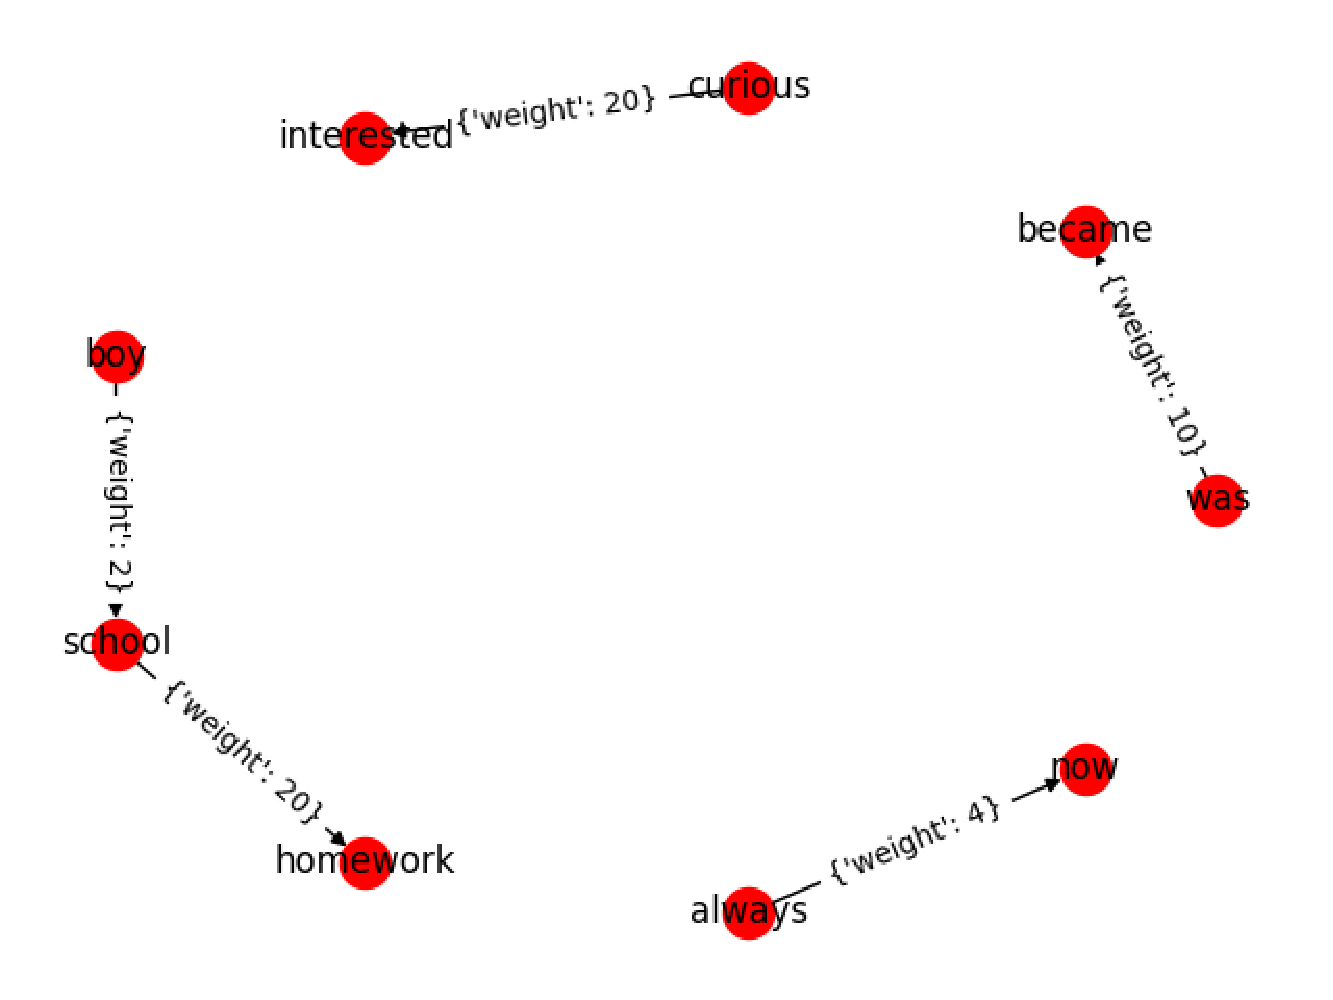
\includegraphics[width=\textwidth]{word_similarity.eps}
\caption{Word \textit{similarity}}
\end{subfigure}
\begin{subfigure}{0.5\textwidth}
\renewcommand\thesubfigure{\roman{subfigure}}
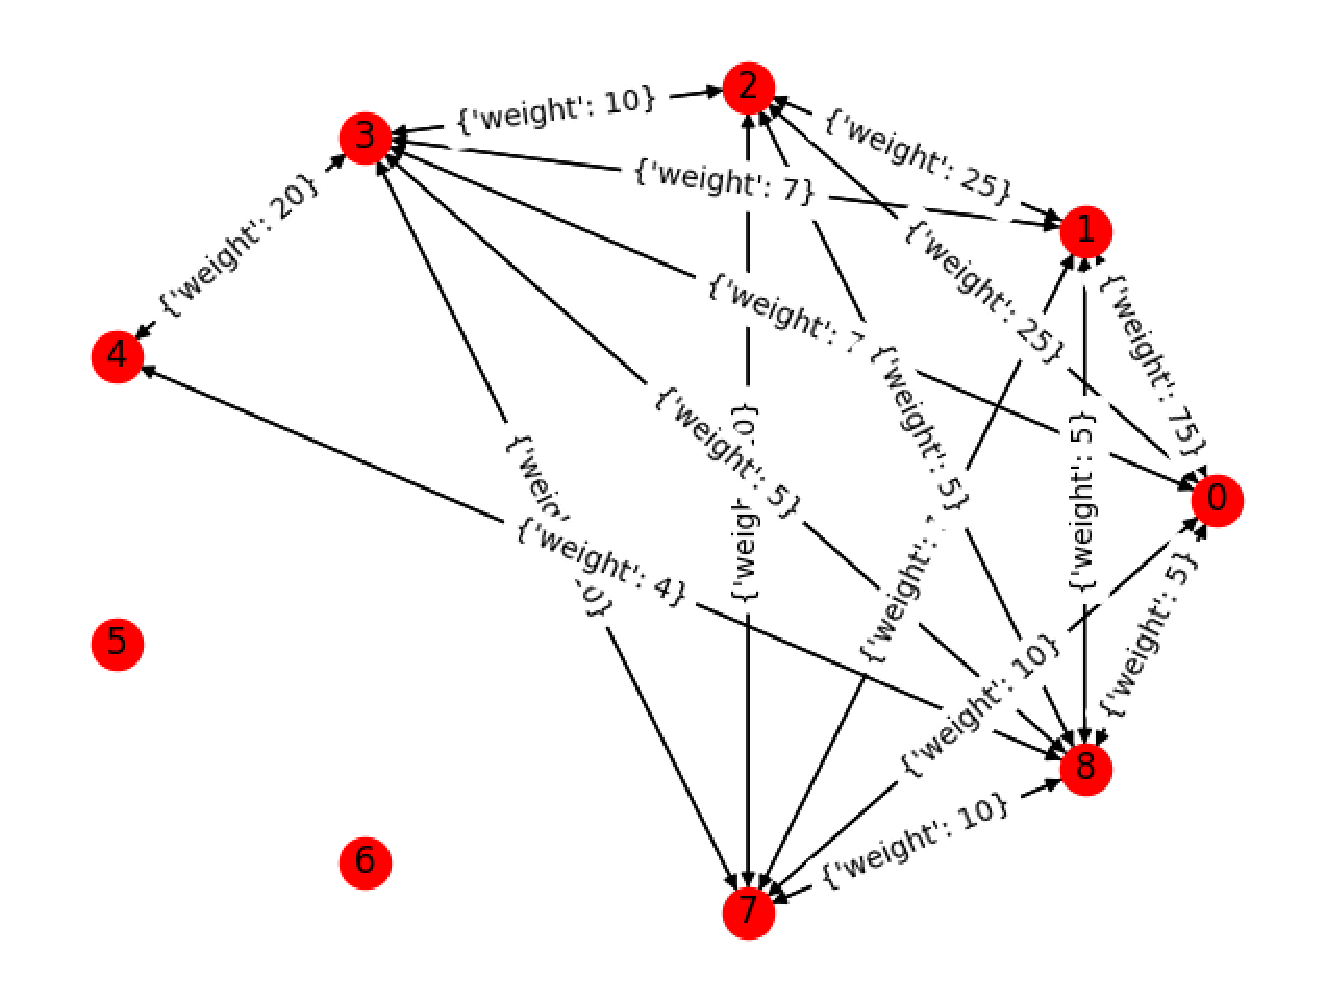
\includegraphics[width=\textwidth]{sentence_similarity.eps}
\caption{Sentence \textit{similarity}}
\end{subfigure}
\setcounter{subfigure}{0}
\caption{\textit{Text relationship maps}}
\label{fig:trm_peter_little}
\end{subfigure}
\begin{subfigure}{\textwidth}
\vspace{\baselineskip}
\centering
\begin{tabular}{@{}llllllllll@{}}
\toprule
Sentence   & 0    & 1    & 2    & 3    & 7    & 8    & 4 & 5 & 6 \\ \midrule
Importance & 40.7 & 24.4 & 18.8 & 14.8 & 12.5 & 11.3 & 6 & 0 & 0 \\ \bottomrule
\end{tabular}
\caption{Sentences ordered by importance}
\end{subfigure}
\begin{subfigure}{\textwidth}
\vspace{\baselineskip}
\begin{displayquote}
there was a curious little boy. the curious little boy was named PeterLittle. PeterLittle was curious in astronomy. PeterLittle was serious in school. PeterLittle did school always. PeterLittle became a astrophysicist. PeterLittle is famous now.
\end{displayquote}
\caption{\textit{Homogenised} story and output of the \textsc{Preprocessor}}
\end{subfigure}
\caption{Example of applying sentence pruning and \textit{homogenisation} to the \textit{simplified} story of Peter Little}
\label{fig:pruning_homogenisation_example}
\end{figure}